
\subsection{Statement}

This section deals with the steady state version of the problem proposed by Smith and Hutton (1982) described in \cite{smith1982numerical}. The problem takes place in the domain $\Omega = (-L,L) \times (0,L) \subset \real^2$ where $L > 0$ is a constant. Both density and diffusion coefficient are assumed to be constant and known values. In $\Omega$ the steady state version of the general convection--diffusion equation with no source term is considered, that is,
\begin{equation}
	\frac{\rho}{\Gamma} \vb{v} \vdot \grad{\phi} = \Delta{\phi}
\end{equation}
On the boundary of $\Omega$ the following conditions are prescribed:
\begin{itemize}[topsep=0pt]
	\item $\phi = 1 + \tanh(10(2x+1))$ on $[-L,0] \times \{ 0 \}$ (inlet flow).
	\item $\dfrac{\partial \phi}{\partial y} = 0$ on $(0,L] \times \{ 0 \}$ (outlet flow).
	\item $\phi = 1 - \tanh(10)$ on $\{ -L \} \times (0,L) \cup [-L,L] \times \{ L \} \cup \{ L \} \times (0,L)$.
\end{itemize}
The velocity field is given by $v_x = 2 y (1 - x^2)$ and $v_y = -2 x (1 - y^2)$, which verifies the incompressibility condition since $\div{\vb{v}} = 0$. The Cauchy problem is the following:
\begin{equation} \label{eq:smith_hutton_cauchy_problem}
	\left\{
	\begin{aligned}
		&\Delta \phi - \frac{\rho}{\Gamma} \vb{v} \vdot \grad{\phi} = 0 &
		&\text{in } \Omega = (0,L) \times (0,L) \\
		&\phi = 1 + \tanh(10(2x+1)) & 
		&\text{on } [-L,0] \times \{ 0 \} \\
		&\frac{\partial \phi}{\partial y} = 0 & 
		&\text{on } (0,L] \times \{ 0 \} \\
		&\phi = 1 - \tanh(10) & 
		&\text{on } \{ -L \} \times (0,L) \cup [-L,L] \times \{ L \} \cup \{ L \} \times (0,L)
	\end{aligned}
	\right.
\end{equation}
Problem \eqref{eq:smith_hutton_cauchy_problem} is summarized in figure \ref{fig:smith_hutton_cauchy_problem}.

\begin{figure}[h]
	\centering
	\begin{tikzpicture}
		% Lenghts
		\def\alength{5}
		\def\L{4.5}
		\def\mlength{0.1}
		% Domain
		\fill[cyan!70!white] (-\L,0) rectangle (\L, \L);
		\draw[thick, thick] (-\L,0) rectangle (\L, \L);
		% Axis
		\draw[-stealth] (-\alength,0) -- (\alength,0) node[above]{$x$};
		\draw[-stealth] (0,-0.5) -- (0,\alength) node[right]{$y$};
		\draw[black, thick] (\L,0) -- ++(0,-\mlength) node[below]{$L$};
		\draw[black, thick] (-\L,0) -- ++(0,-\mlength) node[below]{$-L$};
		\draw[black, thick] (0,\L) -- ++(-\mlength,0) node[left, yshift=2mm]{$L$};
		% Right boundary condition
		\node[inner sep=0pt] at (\L,{0.5*\L}) (rb) {};
		\node[] at ({\L+2},{0.5*\L+1}) (rbc) {$\phi = 1 - \tanh(10)$};
		\path[-latex] (rbc) edge[bend left] node [left] {} (rb);
		% Top boundary condition
		\node[inner sep=0pt] at ({0.1*\L},\L) (tb) {};
		\node[] at ({0.1*\L+2},{\L+1}) (tbc) {$\phi = 1 - \tanh(10)$};
		\path[-latex] (tbc) edge[bend right] node [left] {} (tb);
		% Left boundary condition
		\node[inner sep=0pt] at (-\L,{0.5*\L}) (lb) {};
		\node[] at (-\L-2,{0.5*\L-1}) (lbc) {$\phi = 1 - \tanh(10)$};
		\path[-latex] (lbc) edge[bend left] node [left] {} (lb);
		% Right bottom boundary condition
		\node[inner sep=0pt] at ({0.5*\L},0) (bb) {};
		\node[] at ({0.5*\L-1},-1) (bbc) {$\dfrac{\partial \phi}{\partial y} = 0$};
		\path[-latex] (bbc) edge[bend right] node [left] {} (bb);
		% Left bottom boundary condition
		\node[inner sep=0pt] at ({-0.5*\L},0) (lbb) {};
		\node[] at ({-0.5*\L-1},-1) (lbbc) {$\phi = 1 + \tanh(10(2x+1))$};
		\path[-latex] (lbbc) edge[bend right] node [left] {} (lbb);
		% PDE outer sep=0pt, greenNode, yshift=3mm, fill=white
		\node[fill=cyan!70!white] at (0,{0.5*\L}) 
		{$\Delta{\phi} - \beta \left( \pdv{\phi}{x} + \pdv{\phi}{x} \right) = 0$};
		% Inlet and outlet
		\node[] at ({-0.5*\L},0.3) {Inlet};
		\node[] at ({0.5*\L},0.3) {Outlet};
	\end{tikzpicture}
	\caption{Cauchy problem for the diagonal flow case.}
	\label{fig:smith_hutton_cauchy_problem}
\end{figure}


\begin{figure}[h]
	\centering
	%	\fbox{% GNUPLOT: LaTeX picture with Postscript
\begingroup
  % Encoding inside the plot.  In the header of your document, this encoding
  % should to defined, e.g., by using
  % \usepackage[cp1252,<other encodings>]{inputenc}
  \inputencoding{cp1252}%
  \makeatletter
  \providecommand\color[2][]{%
    \GenericError{(gnuplot) \space\space\space\@spaces}{%
      Package color not loaded in conjunction with
      terminal option `colourtext'%
    }{See the gnuplot documentation for explanation.%
    }{Either use 'blacktext' in gnuplot or load the package
      color.sty in LaTeX.}%
    \renewcommand\color[2][]{}%
  }%
  \providecommand\includegraphics[2][]{%
    \GenericError{(gnuplot) \space\space\space\@spaces}{%
      Package graphicx or graphics not loaded%
    }{See the gnuplot documentation for explanation.%
    }{The gnuplot epslatex terminal needs graphicx.sty or graphics.sty.}%
    \renewcommand\includegraphics[2][]{}%
  }%
  \providecommand\rotatebox[2]{#2}%
  \@ifundefined{ifGPcolor}{%
    \newif\ifGPcolor
    \GPcolortrue
  }{}%
  \@ifundefined{ifGPblacktext}{%
    \newif\ifGPblacktext
    \GPblacktextfalse
  }{}%
  % define a \g@addto@macro without @ in the name:
  \let\gplgaddtomacro\g@addto@macro
  % define empty templates for all commands taking text:
  \gdef\gplbacktext{}%
  \gdef\gplfronttext{}%
  \makeatother
  \ifGPblacktext
    % no textcolor at all
    \def\colorrgb#1{}%
    \def\colorgray#1{}%
  \else
    % gray or color?
    \ifGPcolor
      \def\colorrgb#1{\color[rgb]{#1}}%
      \def\colorgray#1{\color[gray]{#1}}%
      \expandafter\def\csname LTw\endcsname{\color{white}}%
      \expandafter\def\csname LTb\endcsname{\color{black}}%
      \expandafter\def\csname LTa\endcsname{\color{black}}%
      \expandafter\def\csname LT0\endcsname{\color[rgb]{1,0,0}}%
      \expandafter\def\csname LT1\endcsname{\color[rgb]{0,1,0}}%
      \expandafter\def\csname LT2\endcsname{\color[rgb]{0,0,1}}%
      \expandafter\def\csname LT3\endcsname{\color[rgb]{1,0,1}}%
      \expandafter\def\csname LT4\endcsname{\color[rgb]{0,1,1}}%
      \expandafter\def\csname LT5\endcsname{\color[rgb]{1,1,0}}%
      \expandafter\def\csname LT6\endcsname{\color[rgb]{0,0,0}}%
      \expandafter\def\csname LT7\endcsname{\color[rgb]{1,0.3,0}}%
      \expandafter\def\csname LT8\endcsname{\color[rgb]{0.5,0.5,0.5}}%
    \else
      % gray
      \def\colorrgb#1{\color{black}}%
      \def\colorgray#1{\color[gray]{#1}}%
      \expandafter\def\csname LTw\endcsname{\color{white}}%
      \expandafter\def\csname LTb\endcsname{\color{black}}%
      \expandafter\def\csname LTa\endcsname{\color{black}}%
      \expandafter\def\csname LT0\endcsname{\color{black}}%
      \expandafter\def\csname LT1\endcsname{\color{black}}%
      \expandafter\def\csname LT2\endcsname{\color{black}}%
      \expandafter\def\csname LT3\endcsname{\color{black}}%
      \expandafter\def\csname LT4\endcsname{\color{black}}%
      \expandafter\def\csname LT5\endcsname{\color{black}}%
      \expandafter\def\csname LT6\endcsname{\color{black}}%
      \expandafter\def\csname LT7\endcsname{\color{black}}%
      \expandafter\def\csname LT8\endcsname{\color{black}}%
    \fi
  \fi
    \setlength{\unitlength}{0.0500bp}%
    \ifx\gptboxheight\undefined%
      \newlength{\gptboxheight}%
      \newlength{\gptboxwidth}%
      \newsavebox{\gptboxtext}%
    \fi%
    \setlength{\fboxrule}{0.5pt}%
    \setlength{\fboxsep}{1pt}%
    \definecolor{tbcol}{rgb}{1,1,1}%
\begin{picture}(7370.00,3968.00)%
    \gplgaddtomacro\gplbacktext{%
      \csname LTb\endcsname%%
      \put(814,719){\makebox(0,0)[r]{\strut{}0.0}}%
      \put(814,1234){\makebox(0,0)[r]{\strut{}0.2}}%
      \put(814,1748){\makebox(0,0)[r]{\strut{}0.4}}%
      \put(814,2263){\makebox(0,0)[r]{\strut{}0.6}}%
      \put(814,2777){\makebox(0,0)[r]{\strut{}0.8}}%
      \put(814,3292){\makebox(0,0)[r]{\strut{}1.0}}%
      \put(946,499){\makebox(0,0){\strut{}-1.0}}%
      \put(2233,499){\makebox(0,0){\strut{}-0.5}}%
      \put(3520,499){\makebox(0,0){\strut{}0.0}}%
      \put(4806,499){\makebox(0,0){\strut{}0.5}}%
      \put(6093,499){\makebox(0,0){\strut{}1.0}}%
    }%
    \gplgaddtomacro\gplfronttext{%
      \csname LTb\endcsname%%
      \put(209,2005){\rotatebox{-270}{\makebox(0,0){\strut{}$y \ (\mathrm{m})$}}}%
      \put(3519,169){\makebox(0,0){\strut{}$x \ (\mathrm{m})$}}%
      \csname LTb\endcsname%%
      \put(6611,719){\makebox(0,0)[l]{\strut{}0.0}}%
      \put(6611,1362){\makebox(0,0)[l]{\strut{}0.5}}%
      \put(6611,2005){\makebox(0,0)[l]{\strut{}1.0}}%
      \put(6611,2648){\makebox(0,0)[l]{\strut{}1.5}}%
      \put(6611,3292){\makebox(0,0)[l]{\strut{}2.0}}%
      \put(7073,2005){\rotatebox{-270}{\makebox(0,0){\strut{}$\phi$}}}%
      \put(3519,3622){\makebox(0,0){\strut{}\textbf{Smith--Hutton case} $(\mathrm{Pe} = 10^{2})$}}%
    }%
    \gplbacktext
    \put(0,0){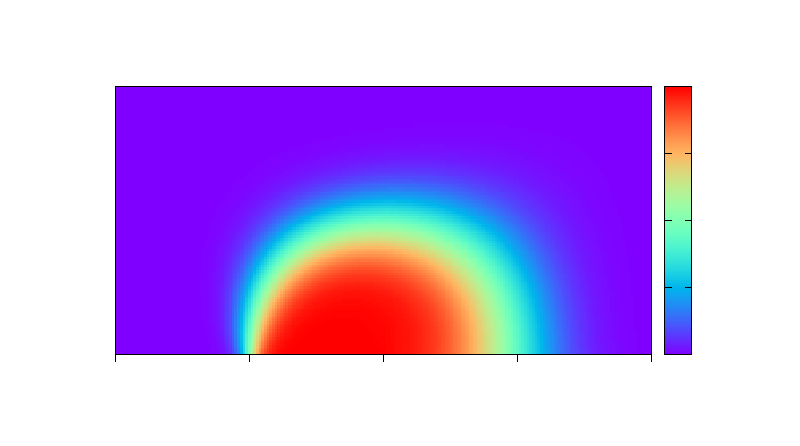
\includegraphics[width={368.50bp},height={198.40bp}]{figures/case_smith_hutton/smith_hutton_N201_Pe1.0e+02}}%
    \gplfronttext
  \end{picture}%
\endgroup
}
	% GNUPLOT: LaTeX picture with Postscript
\begingroup
  % Encoding inside the plot.  In the header of your document, this encoding
  % should to defined, e.g., by using
  % \usepackage[cp1252,<other encodings>]{inputenc}
  \inputencoding{cp1252}%
  \makeatletter
  \providecommand\color[2][]{%
    \GenericError{(gnuplot) \space\space\space\@spaces}{%
      Package color not loaded in conjunction with
      terminal option `colourtext'%
    }{See the gnuplot documentation for explanation.%
    }{Either use 'blacktext' in gnuplot or load the package
      color.sty in LaTeX.}%
    \renewcommand\color[2][]{}%
  }%
  \providecommand\includegraphics[2][]{%
    \GenericError{(gnuplot) \space\space\space\@spaces}{%
      Package graphicx or graphics not loaded%
    }{See the gnuplot documentation for explanation.%
    }{The gnuplot epslatex terminal needs graphicx.sty or graphics.sty.}%
    \renewcommand\includegraphics[2][]{}%
  }%
  \providecommand\rotatebox[2]{#2}%
  \@ifundefined{ifGPcolor}{%
    \newif\ifGPcolor
    \GPcolortrue
  }{}%
  \@ifundefined{ifGPblacktext}{%
    \newif\ifGPblacktext
    \GPblacktextfalse
  }{}%
  % define a \g@addto@macro without @ in the name:
  \let\gplgaddtomacro\g@addto@macro
  % define empty templates for all commands taking text:
  \gdef\gplbacktext{}%
  \gdef\gplfronttext{}%
  \makeatother
  \ifGPblacktext
    % no textcolor at all
    \def\colorrgb#1{}%
    \def\colorgray#1{}%
  \else
    % gray or color?
    \ifGPcolor
      \def\colorrgb#1{\color[rgb]{#1}}%
      \def\colorgray#1{\color[gray]{#1}}%
      \expandafter\def\csname LTw\endcsname{\color{white}}%
      \expandafter\def\csname LTb\endcsname{\color{black}}%
      \expandafter\def\csname LTa\endcsname{\color{black}}%
      \expandafter\def\csname LT0\endcsname{\color[rgb]{1,0,0}}%
      \expandafter\def\csname LT1\endcsname{\color[rgb]{0,1,0}}%
      \expandafter\def\csname LT2\endcsname{\color[rgb]{0,0,1}}%
      \expandafter\def\csname LT3\endcsname{\color[rgb]{1,0,1}}%
      \expandafter\def\csname LT4\endcsname{\color[rgb]{0,1,1}}%
      \expandafter\def\csname LT5\endcsname{\color[rgb]{1,1,0}}%
      \expandafter\def\csname LT6\endcsname{\color[rgb]{0,0,0}}%
      \expandafter\def\csname LT7\endcsname{\color[rgb]{1,0.3,0}}%
      \expandafter\def\csname LT8\endcsname{\color[rgb]{0.5,0.5,0.5}}%
    \else
      % gray
      \def\colorrgb#1{\color{black}}%
      \def\colorgray#1{\color[gray]{#1}}%
      \expandafter\def\csname LTw\endcsname{\color{white}}%
      \expandafter\def\csname LTb\endcsname{\color{black}}%
      \expandafter\def\csname LTa\endcsname{\color{black}}%
      \expandafter\def\csname LT0\endcsname{\color{black}}%
      \expandafter\def\csname LT1\endcsname{\color{black}}%
      \expandafter\def\csname LT2\endcsname{\color{black}}%
      \expandafter\def\csname LT3\endcsname{\color{black}}%
      \expandafter\def\csname LT4\endcsname{\color{black}}%
      \expandafter\def\csname LT5\endcsname{\color{black}}%
      \expandafter\def\csname LT6\endcsname{\color{black}}%
      \expandafter\def\csname LT7\endcsname{\color{black}}%
      \expandafter\def\csname LT8\endcsname{\color{black}}%
    \fi
  \fi
    \setlength{\unitlength}{0.0500bp}%
    \ifx\gptboxheight\undefined%
      \newlength{\gptboxheight}%
      \newlength{\gptboxwidth}%
      \newsavebox{\gptboxtext}%
    \fi%
    \setlength{\fboxrule}{0.5pt}%
    \setlength{\fboxsep}{1pt}%
    \definecolor{tbcol}{rgb}{1,1,1}%
\begin{picture}(7370.00,3968.00)%
    \gplgaddtomacro\gplbacktext{%
      \csname LTb\endcsname%%
      \put(814,719){\makebox(0,0)[r]{\strut{}$0$}}%
      \put(814,1234){\makebox(0,0)[r]{\strut{}$0.2$}}%
      \put(814,1748){\makebox(0,0)[r]{\strut{}$0.4$}}%
      \put(814,2263){\makebox(0,0)[r]{\strut{}$0.6$}}%
      \put(814,2777){\makebox(0,0)[r]{\strut{}$0.8$}}%
      \put(814,3292){\makebox(0,0)[r]{\strut{}$1$}}%
      \put(946,499){\makebox(0,0){\strut{}-1.0}}%
      \put(2233,499){\makebox(0,0){\strut{}-0.5}}%
      \put(3520,499){\makebox(0,0){\strut{}0.0}}%
      \put(4806,499){\makebox(0,0){\strut{}0.5}}%
      \put(6093,499){\makebox(0,0){\strut{}1.0}}%
    }%
    \gplgaddtomacro\gplfronttext{%
      \csname LTb\endcsname%%
      \put(209,2005){\rotatebox{-270}{\makebox(0,0){\strut{}$y \ (\mathrm{m})$}}}%
      \put(3519,169){\makebox(0,0){\strut{}$x \ (\mathrm{m})$}}%
      \csname LTb\endcsname%%
      \put(6611,719){\makebox(0,0)[l]{\strut{}0.0}}%
      \put(6611,1362){\makebox(0,0)[l]{\strut{}0.5}}%
      \put(6611,2005){\makebox(0,0)[l]{\strut{}1.0}}%
      \put(6611,2648){\makebox(0,0)[l]{\strut{}1.5}}%
      \put(6611,3292){\makebox(0,0)[l]{\strut{}2.0}}%
      \put(7073,2005){\rotatebox{-270}{\makebox(0,0){\strut{}$\norm{\vb{v}} \ (\mathrm{m} / \mathrm{s})$}}}%
      \put(3519,3622){\makebox(0,0){\strut{}\textbf{Smith--Hutton case -- Velocity field}}}%
    }%
    \gplbacktext
    \put(0,0){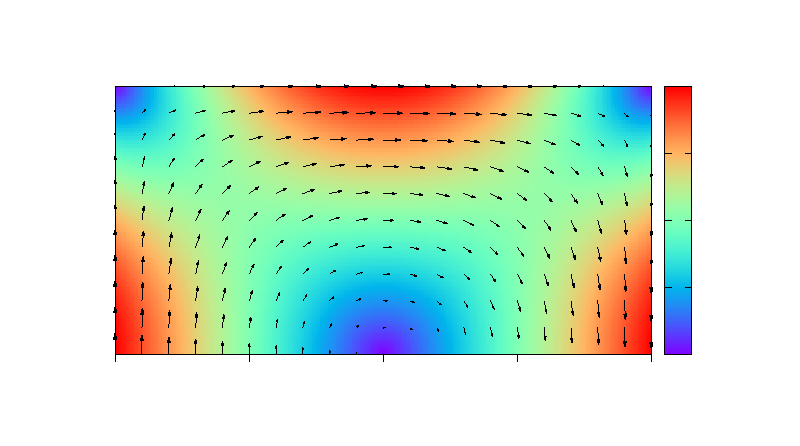
\includegraphics[width={368.50bp},height={198.40bp}]{figures/case_smith_hutton/smith_hutton_velocity_field}}%
    \gplfronttext
  \end{picture}%
\endgroup

	\caption{}
	\label{fig:smith_hutton_velocity_field}
\end{figure}


